\documentclass[12pt]{article}
\usepackage[margin=1in]{geometry} 
\usepackage{amsmath,amsthm,amssymb,amsfonts}
\usepackage{graphicx}
\usepackage{authblk}
\usepackage{todonotes}
\usepackage{hyperref}
\usepackage{listings}
\usepackage{float}


\newcommand{\N}{\mathbb{N}}
\newcommand{\Z}{\mathbb{Z}}
\newcommand{\Q}{\mathbb{Q}}
 
\newenvironment{problem}[2][problem]{\begin{trivlist}
\item[\hskip \labelsep {\bfseries #1}\hskip \labelsep {\bfseries #2.}]}{\end{trivlist}}
 
\begin{document}
\lstset{language=Python}
 
\title{\textbf{Dog Breed Identification Using Machine Learning Classification Techniques}}
\date{}

\author{
        Kaitlyn Mulligan\\
        Marist College - DATA 440L \\
        May 15, 2019
 }

\maketitle

\begin{abstract}
    Machine learning is a growing field that has greatly increased with the continuing advancements in technology.  This area provides many tools that can all perform different tasks on large data sets.  The focus of this paper is on classification tools.  Classification tools are utilized in order to classify or predict the breeds of dogs based on an input image.  Many methods are used in attempts to classify the images in the dataset.  The dataset comes from a Kaggle competition in which the goal is to predict the breed of dog in the image.  Participants tried many different methods, some of which helped inspire this project.  The classification tools that are explored here are a Convolutional Neural Network and Xception with a Multilayer Perceptron.  The paper explores the trial and error in all of the methods as well as the final model that was used to predict and classify the dog breeds.  While the final model has a much better prediction rate than the original attempt, there is an acknowledgement of the errors made throughout the process.  With this acknowledgement comes areas to improve and ideas to further explore and improve this program as a classification tool on dog breeds.
\end{abstract} \hspace{10pt}
\thispagestyle{empty}
\clearpage
\setcounter{page}{1}

\section{Introduction}
\quad Machine learning is a widely growing field.  Continued advancements in technology have greatly impacted the development of machine learning, allowing the field to gain increased momentum, as it continues to grow.  Data analysis can take humans potentially only a few minutes, but it could also take a very long time.  Machine learning allows data analyses to be performed by the computer in place of humans.  Although some machine learning algorithms have been around for some time, we have not always had the abilties with it that we do now.  With current technology and advancements, we have the ``ability to automatically apply complex mathematical calculations to big data - over and over, faster and faster''\cite{SAS}.  Machine learning falls under a branch of artificial intelligence based on the idea that ``systems can learn from data, identify patterns and make decisions with minimal human intervention''\cite{SAS}.  The process that the systems use to learn from the data is an iterative process.  This is important because as the models continue to be exposed to more and more data, it is able to continuously learn from the new data.

My motivation for this project was to learn how to use a classification tool on images in order to classify the image.  To do so, I utilized a dataset which consisted of images of different breeds of dogs.  My goal was to build a program which will learn the different breeds of dogs in order to predict the breed of dog represented in the input image.  While in the process of building this program, I came across many different techniques, of which, I tried a few.  First, I tried to use a Convolutional Neural Network to predict the dog breeds.  After trying a few different settings with the CNN, I decided to then try Logistic Regression using Xception and a Multilayer Perceptron.  Once the optimal model is found, we can analyze the model to see how well it is performing to classify the different dog breeds.  With these results, we can determine where improvements could be made or if different methods should be attempted to further improve the systems ability to predict the dog breeds.

\section{Background and Related Work}
\quad Throughout this process, I analyzed Convolutional Neural Networks and Xception.  Convolutional Neural Networks are gaining popularity when it comes to classifying images, but I wanted to find a method that would better predict the breed of dog.  Therefore, the method I ended up using to predict dog breeds was with Xception and an MLP.  Xception seems like its own method, but in simple terms it is a very large convolutional neural network.  It is ``trained on more than a million images from the ImageNet database''\cite{MathWorks}.  Xception is 71 layers deep and can classify a variety of different images.  Xception is a newer method compared to Inception.  It was named Xception because it is an ``Extreme version of Inception''\cite{Tsang2018}.  With Xception I used a Multilayer Perceptron.  The Multilayer Perceptron is a deep, artificial neural network.  In \cite{Skymind}, they state that ``the multilayer perceptron is the hello world of deep learning: a good place to start when you are learning about deep learning.''

There are many different examples on the internet of how people use different methods to classify images.  In regards to dog breed identification, many people have attempted to make a program that will achieve good results because it was a Kaggle competition.  Many people partcipated in this competition, using a variety of different methods in an attempt to predict the dog breeds.  After viewing some of the participants ideas on how to go about this problem, it seemed that using a Convoutional Neural Network was a fairly popular method.  Participants also used Xception, Inception, and other methods to predict the breeds of dogs.

\section{Methodology}
\quad The process of programming a system to predict the breed of dog in an image required a great deal of trial and error.  I attempted many different things before deciding to use Xception and an MLP to predict the breed of dog in an image.  Initially, I planned to use a Convolutional Neural Network.  During the semester we learned about CNNs and their applications.  I realized that it would be a good method to apply as I attempted to predict dog breeds based on images.  We utilized CNNs to classify images that the students took from around the building.  This dataset included chalk, lights, chairs, and a few other items.  The program we created was able to predict to a certain extent.  From this lesson, I adapted the program to my dataset to try to predict dog breeds.  In using the CNN, I first tried it with two convolutional layers and five full connection layers.  These full connection layers consisted of relu, sigmoid, and dropout.  I then attempted another version of a CNN without any convolutional layers, but ran into some problems with it.  The problems with the CNN will be touched upon in the following section.

For my final project, as mentioned, I utilized Xception and an Multilayered Perceptron.  Before going into the experimentation phase of implementing my program, I will establish some basics of these methods.

Xception utilizes depthwise separable convolutions.  In total there are 36 convolutional stages within this methodology.  The Xception model performs the one by one convolution first, and then moves into the channel wise spatial convolution.  This is depicted by the graphic below.
\begin{center}
     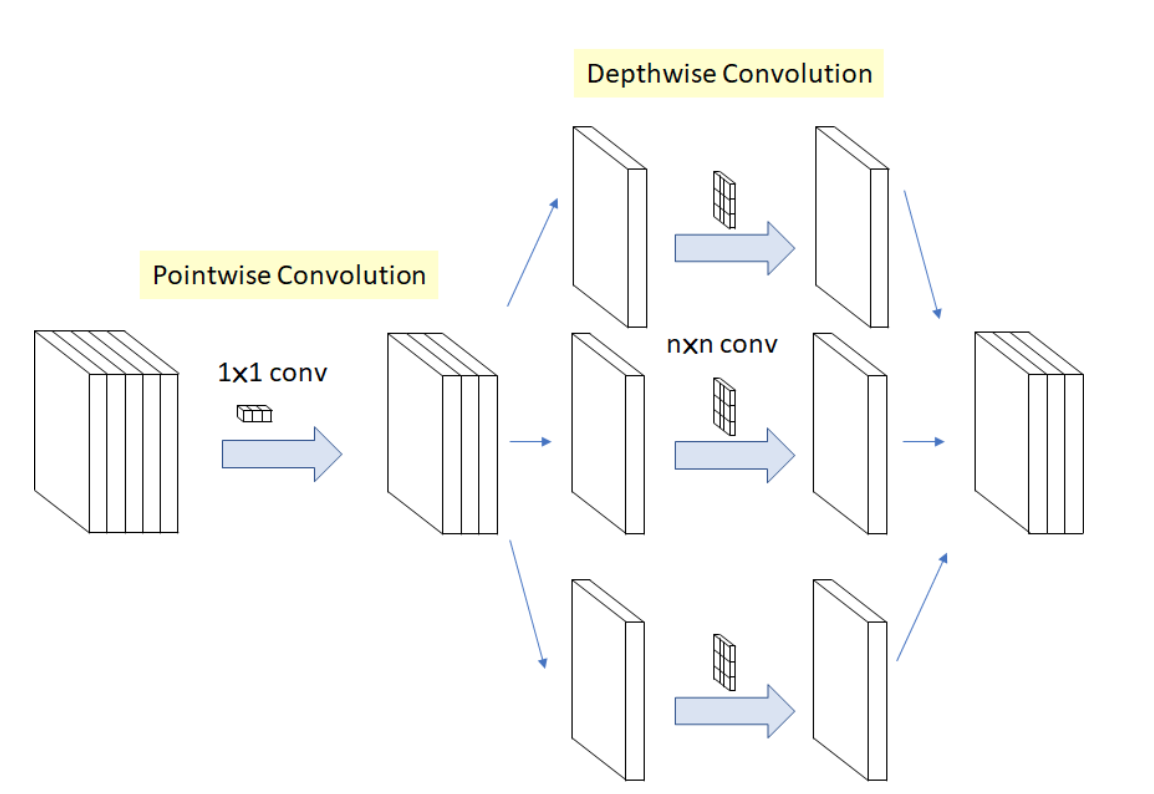
\includegraphics[width=0.5\textwidth]{XceptionModel.jpg}
\end{center}
Xception does not have an intermediate activation.  Due to this, it has the highest accuracy compared to other methods such as Inception.  Lastly, Xception performs better due to the better use of the model parameters.

Briefly descibed earlier, the Multilayer Perceptron is a deep, artificial neural network.  Multilayer Perceptrons are composed of 3 key components.  The first is the input layer.  This is the layer that receives the signal.  Next we have an arbitrary number of hidden layers.  Lastly, we have the output layer.  This is the layer that makes the decision or prediction regarding the input.  A simple model of a Multilayer Perceptron is depicted in the graphic below.
\begin{center}
     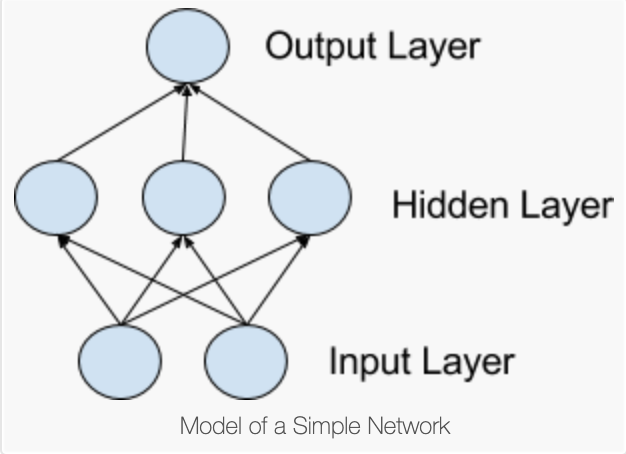
\includegraphics[width=0.4\textwidth]{MLP.jpg}
\end{center}
With the MLP I implemented classification.  The classification provides the results that can be utilized to determine how well the system is performing.  Metrics such as confusion matrices, LogLoss, and Balanced Accuracy Score are all provided as output to understand the performance of the system.

When implementing Xception and the MLP, the data is split into testing and training data.  The model then learns on the training data.  The goal for the system is to obtain a high accuracy rate and minimize the error by adjusting parameters.  With this comes a lot of trial and error which will be explored in the following section.

\section{Experiments}
\subsection{Data}
\quad The dog breed dataset, which was the focus of this project, came from a Kaggle competition in which the task was to determine the breed of a dog based on an image.  The data can be accessed here: \href{https://www.kaggle.com/c/dog-breed-identification}{Dog Breed Identification}.  The data set included a training and testing set of images for different breeds of dogs.  Each image has a filename that corresponds to a unique ID which can be found in the file \verb|labels.csv|.  This file contains the ID which is the filename, and the breed of dog in the image.  A preview of this file is shown below.
\begin{center}
     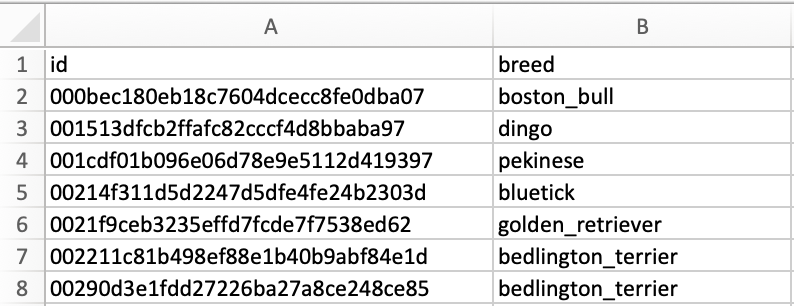
\includegraphics[width=0.5\textwidth]{labels.jpg}
\end{center}
The dataset is comprised of 120 unique dog breeds.  For my program, I only utilized the training dataset provided and from there split it into training and testing sets.  The training dataset included 10,222 images of dogs.

\subsection{Convolutional Neural Network}
\quad To reiterate, my initial idea was to adapt our CNN program from class to my project on predicting dog breeds.  After making the necessary changes to the program, I was able to begin experimenting with it.  I started off with a small number of epochs and a small batch size.  In doing so, I did not obtain very good results.  I realized I had to keep fiddling with the numbers and try bigger and smaller values for the number of epochs and the batch size.  In addition to this, I also tried different combinations of the two.  This still did not give me very good results.  I continued to change things around and moved on to trying different full connections layers.  I did not initially have dropout layers in my CNN so I tried to add some of those in.  Once changing my full connection layers, I continued to change around the number of epochs and the batch size to see if I could improve my results.  After trying to predict some dog breeds, I realized that the program was greatly overfitting the data.  Overall, with the CNN I was working with initially, the highest prediciton rate I obtained was 10\%.  After consulting my professor, we decided to change some more aspects of the CNN.  We changed more parameters and got rid of convolutional layers.  After a lot of work to try and make this work, we kept obtaining errors.  Since time was beginning to run out, we decided to try Xception and MLP instead.

\subsection{Xception and MLP}
\quad When implementing this new method to predict dog breeds, the first step I needed was to load Xception and split the data into training and testing sets.  With the data split, I then needed to run the training and testing sets through Xception.  In my model, I needed to learn which set of neurons along with what value of $\eta$ would provide me with the best model to predict dog breeds.  These values are not known without running the program to see what the cross validation score is and comparing it amongst others.  Therefore, I created a for loop within a for loop.  I utilized eight different sets of neurons and four different values of $\eta$.  At the end of each for loop run through, the cross validation score would be compared against the current, best cross validation score.  If it was better, these new values would be stored, but if it was not better it would move on to the next set of neurons or the next value of $\eta$.  Ideally, once all of the sets of neurons and values of $\eta$ were scanned through, we would have a final, best model to use for predicions.

Of course, the ideal case does not always occur.  Before running the program with all the sets of neurons and value of $\eta$, I wanted to make sure the program itself worked.  Therefore, I decided to run it with only two sets of neurons and two values of $\eta$ initially.  This proved to be a good idea as even with this small amount of values the program is scanning through, it took three hours to complete.  At the end of the first run through of this program, I obtained an error and went back through and fixed it.  I continued to use only two sets of neurons and two values of $\eta$ until I was sure that the whole program worked.  Once I was ensured that it worked I could move on to run the program with all of the sets of neurons and values of $\eta$ to determine which out of all of them created the best model to predict dog breeds.

The problems were not yet over though.  As I learned in my attempt to run the program with all of the sets of neurons and values of $\eta$, it takes a very long time to complete and Google Colab runtime disconnects after sitting idle for awhile.  Thus, I was never able to run the full program at once.  I needed to break it down more so that it did not take as long.  This would allow me to record all of my observations and compare them all in the end.  When comparing the results in the end, I examined the cross validation scores and not the balanced accuracy score.  I looked for the highest cross validation score because utilizing cross validation takes into consideration and helps control overfitting.  I did not look for the highest balanced accuracy score because this value was not being run through cross validation, therefore, this value should not be trusted as a truly accurate representation of the prediction accuracy.  Looking for the highest cross validation score out of all of the results I obtained, I found that the set of neurons (400, 200) and $\eta$ being 0.001 would produce the best model for the classification of dog breeds.  Once these values were saved, I no longer needed to run the entire model.  Instead, I was able to just run the MLP Classification with these hyperparameters to obtain the performance metrics which will be analyzed in the following section.

\section{Discussion and Analysis}
\quad In order to analyze the performance of the model I have created, I needed to run performance metrics.  The performance metrics I obtained included confusion matrices, LogLoss, and Accuracy.  The confusion matrices show us how well the model was trained and how well the model predicted on the test data set.  It compares the true dog breed to the predicted dog breed regarding specific images.  For my optimal model I obtained the following confusion matrices for the training and testing datasets.
\begin{figure}[H]
    \begin{minipage}{0.45\textwidth}
        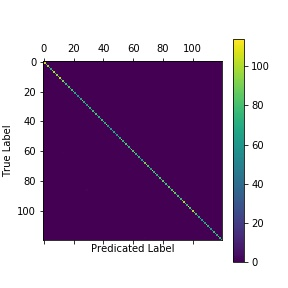
\includegraphics[width=0.9\textwidth]{confusion_matrix_train.jpg}
        \caption{Training Confusion Matrix}
    \end{minipage}\hfill
    \begin{minipage}{0.45\textwidth}
        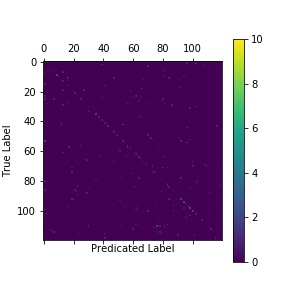
\includegraphics[width=0.9\textwidth]{confusion_matrix_test.jpg}
        \caption{Testing Confusion Matrix}
    \end{minipage}
\end{figure}
As you can see, the model is doing a good job training as there is a clear diagonal line which represents the true breed matching the predicted breed.  Then analyzing the testing confusion matrix, we can see that the diagonal line, which represents the accurate predictions, is not as prevalent.  Instead, we can see that there are scattered dots throughout the rest of the confusion matrix, which represent incorrect predictions.

The testing LogLoss and Accuracy were also reported.  These measures are not a good representation of the true rates of LogLoss and Accuracy becuase they are not being passed through cross validation, but they provide a good idea of how the system is performing.  The optimal model produced a LogLoss of 10.7656 and an Accuracy of 0.5349, or 53.49\%.  In the future uses of my system, I plan on editing the LogLoss and Accuracy so that they are running through cross validation in order to obtain a better representation of these values.  Another aspect of this program that should be editied in the future is the number of splits.  The results obtained here were only run on three splits due to time constraints.  Running the program with ten splits will allow the program to train more and potentially increase the prediction rate.

With these performance metrics in mind, attempts to predict dog breeds can be made.  One way that predictions can be made are on the test data set that we split the data into at the beginning.  This is passing in an image that is from the data set and see what the system predicts it as.  To determine this, I analyzed the predictive probability and looked for the maximum value in the array.  The maximum value represents the index of the dog breed predicted.  Since this input image is an image from the original data set, we are able to obtain the true value of the dog breed in the image.  Comparing the value that the system outputted against the true value, we can determine if the system predicted that specific image correctly or not.  With the index of the predicted breed, we can also obtain the name of the breed that the system predicted.  This allows us to compare the input image of the dog with what the system predicted it to be.  For example, suppose we are trying to predict the breed of this dog:
\begin{center}
    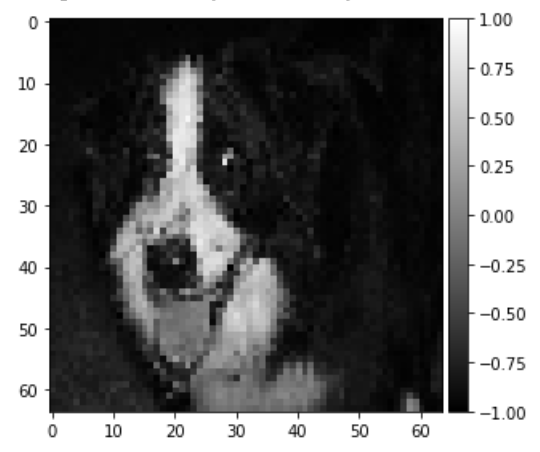
\includegraphics[width=0.4\textwidth]{predictDog.jpg}
\end{center}
The system will return the following array
\begin{center}
    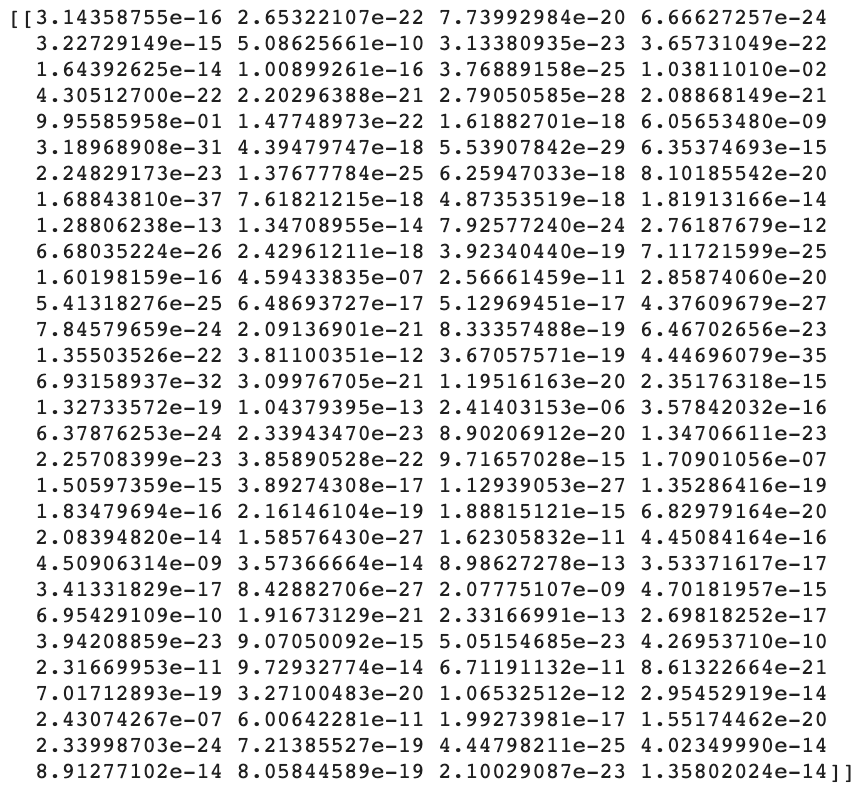
\includegraphics[width=0.4\textwidth]{output.jpg}
\end{center}
The program also outputs the index that has the maximum value.  In this case the value it output was 16.  I have also programmed it to output the true value of the dog breed represented in the image.  In this case, this output was also a 16, indicating that the breed was predicted correctly.

Another way to predict images is by inputting your own images into the system.  For example, I was able to input an image of my dog and see what the system predicted it to be.  The system would again output the probabilities for the image being each breed in the dataset.  As in the last case, taking the maximum value of this gives us which breed the system is predicting for this image.  Using the index, we can determine which breed this is.  Since it is a self-inputted image, and I know the breed of my dog, I am able to determine if it is predicting correctly or not.  Unfortunately, with the image I inputted, it did not predict my dog correctly.  The system predicted an index of 88 for one photo which represents an entlebucher and an index of 82 for a second photo which represents a malamute.  My dog is a Golden Doodle, which, unfortunately, is not very similar to either of these breeds.

\section{Conclusion}
\quad The motivation of this project was to learn how to use a machine learning classification tool in order to classify images, namely, dog breeds.  After trying a few different methods, along with some trial and error, I feel as though I have gained a much deeper understanding of machine learning and classification tools.  Specifically, I feel my ability to work with Convolutional Neural Netowrks, Xception, and Multilayer Perceptrons has greaty increased since the beginning of the project.  Initially, I had very minimal experience using python as well as minimal understanding of what exactly the field of machine learning consisted of.  Through my research and class sessions, I have grown an interest in this field and learning new areas and methods of machine learning.  As stated earlier, due to time constraints, I was unable to perform everything I had envisioned.  Thus, I have summarized a few of my goals I would like to continue to work towards.

In the future, I would like to continue to improve this program to improve the prediction accuracy rate.  One way to potentially do so would be to run it with more sets of neurons and vlaues of $\eta$.  Due to time constraints of this project, I was unable to run it with many sets of neurons and values of $\eta$.  There is a potential this could increase the prediction rate, but this is unknown until further research is performed.  Additionally, to further improve the program I currently have, the MLP Classification, LogLoss score, and Balanced Accuracy score should be run through cross validation.  This would provide a better measure of the actual prediction rate because it takes into consideration overfitting and deals with that inflating or deflating the prediction rate.  Lastly, to improve my current model, I would like to run my program with ten k-folds of cross validaiton instead of three.  For this project, I utilized three folds due to time constraints and how long each took to run.  In the future, I would be interested in seeing how changing that value to ten will change the prediciton rate.  These changes can be made possible because there are no longer time constraints.

Outside of changing the current program I have, I would also be interested in testing other methods abilities to predict the dog breeds.  During this project I have tested a Convolutional Neural Network and Xception.  I am curious as to how other methods work and how the results would or would not improve.  It would be interesting to show how the different methods compare against each other as well.  Additionally, as I was performing my preliminary research about this data set and what participants in this competition did, it seemed a lot of them limited the number of dog breeds they included in their programs.  It would be interesting to test different combinations of a certain number of breeds to see how accuracy could increase or decrease due to this.  This can be greatly impacted depending on if one dog breed is more or less prevalent in the entire data set as compared to other dog breeds.

\begin{thebibliography}{9} 

\bibitem{Skymind}
``A Beginner's Guide to Multilayer Perceptrons (MLP),'' Skymind. [Online]. Available: https://skymind.ai/wiki/multilayer-perceptron. [Accessed: 14-May-2019].

\bibitem{Escontrela2018}
A. Escontrela, ``Convolutional Neural Networks from the ground up,'' \textit{Towards Data Science}, 16-Jun-2018. [Online]. Available: https://towardsdatascience.com/convolutional-neural-networks-from-the-ground-up-c67bb41454e1. [Accessed: 24-Mar-2019].

\bibitem{Kaggle}
``Dog Breed Identification,'' \textit{Kaggle}. [Online]. Available: https://www.kaggle.com/c/dog-breed-identification. [Accessed: 13-Feb-2019].

\bibitem{Bendemra2018}
H. Bendemra, ``Build Your First Deep Learning Classifier using TensorFlow: Dog Breed Example,'' \textit{Towards Data Science}, 26-Apr-2018. [Online]. Available: https://towardsdatascience.com/build-your-first-deep-learning-classifier-using-tensorflow-dog-breed-example-964ed0689430. [Accessed: 24-Mar-2019].

\bibitem{Brownlee2018}
J. Brownlee, ``When to Use MLP, CNN, and RNN Neural Networks,'' Machine Learning Mastery, 23-Jul-2018. [Online]. Available: https://machinelearningmastery.com/when-to-use-mlp-cnn-and-rnn-neural-networks/. [Accessed: 08-May-2019].

\bibitem{SAS}
``Machine Learning: What it is and why it matters,'' SAS. [Online]. Available: https://www.sas.com/en\_us/insights/analytics/machine-learning.html. [Accessed: 14-May-2019].

\bibitem{Tsang2018}
S.-H. Tsangm ``Review: Xception - With Depthwise Separable Convolution, Better Than Inception-v3 (Image Classification),'' Towards Data Science, 25-Sep-2018. [Online]. Available: https://towardsdatascience.com/review-xception-with-depthwise-separable-convolution-better-than-inception-v3-image-dc967dd42568. [Accessed: 14-May-2019].

\bibitem{MathWorks}
``Xception,'' MathWorks. [Online]. Available: https://www.mathworks.com/help/\\deeplearning/ref/xception.html. [Accessed: 14-May-2019].

\end{thebibliography}

\end{document}